\chapter{Clean Architecture}

\section{Was ist Clean Architecture?}

Clean Architecture ist ein allgemeines Konzept zum Design von Softwarearchitekturen, das darauf abzielt, 
die Struktur einer Anwendung so zu gestalten, dass sie unabhängig von ihren Benutzerschnittstellen, 
Datenquellen und anderen äußeren Faktoren bleibt. 
Dies bedeutet, dass die verschiedenen Komponenten 
und Funktionen einer Anwendung in abgekapselten Schichten angeordnet werden (\textit{Onion}-Architektur), 
um sicherzustellen, dass Veränderungen in einer Schicht die tieferliegenden Schichten nicht beeinflussen. 
Außere Schichten haben dabei Abhängigkeiten von tieferen Schichten aber niemals umgekehrt.
Aufrufe von tieferen Schichten an äußere Schichten werden über Abstraktionen (\textit{Dependency Inversion} und 
\textit{Injection}) realisiert. Tiefere Schichten sind dabei langlebiger als Schichten weiter außen. \\
Dies führt zu einer Anwendung, die flexibler und leichter zu entwickeln und zu warten ist, 
da Änderungen an einem Teil der Anwendung die tieferliegenden Schichten nicht berühren.

\section{Analyse der Dependency Rule}

Schichten im Sinne der Dependency Rule sind hierp \texttt{plugin}, \texttt{application}, \texttt{domain} 
und \texttt{abstraction} aufsteigend geordnet nach zunehmender Tiefe in der Onion-Architektur\footnote{Siehe \autoref{sec:clean_arch_layers} für mehr Informationen.}. 
Sie werden durch gleichnamige Packages, die parallel unter \\ 
\texttt{de.dhbw.karlsruhe.ase} \\
zu finden sind, erschöpfend repräsentiert. 
Es sind Abhängigkeiten von äußerden Schichten in tiefere Schichten erlaubt, aber nicht umgekehrt.
Diese Regel wird für die oben genannten Schichten \underline{immer} eingehalten, 
was die folgenden beiden Beispiele illustrieren.  

\subsubsection{Positiv-Beispiel 1:}

\autoref{fig:dep-camp} zeigt das verlangte UML-Diagramm der Beispielklasse 1 \textit{Camp} der Schicht \textit{domain}, 
welches die Dependency Rule einhält. Wie im Diagramm zu sehen ist hängt Camp ausschließlich von 
Klassen in der selben Schicht (\textit{domain}) ab. 
\textit{Crafting} ist dabei keine Schicht sondern ein \textit{Aggregat}\footnote{Siehe \autoref{sec:ddd}.}. 
Schichten sind ausschließlich die oben genannten. \\ 
Weiter zu sehen ist, dass ausschließlich Klassen in \textit{application} von Camp abhängen, aber keine 
aus höheren Schichten (was in diesem konkreten Fall nur \textit{abstraction} sein könnte).

\begin{figure}[H]
	\centering
	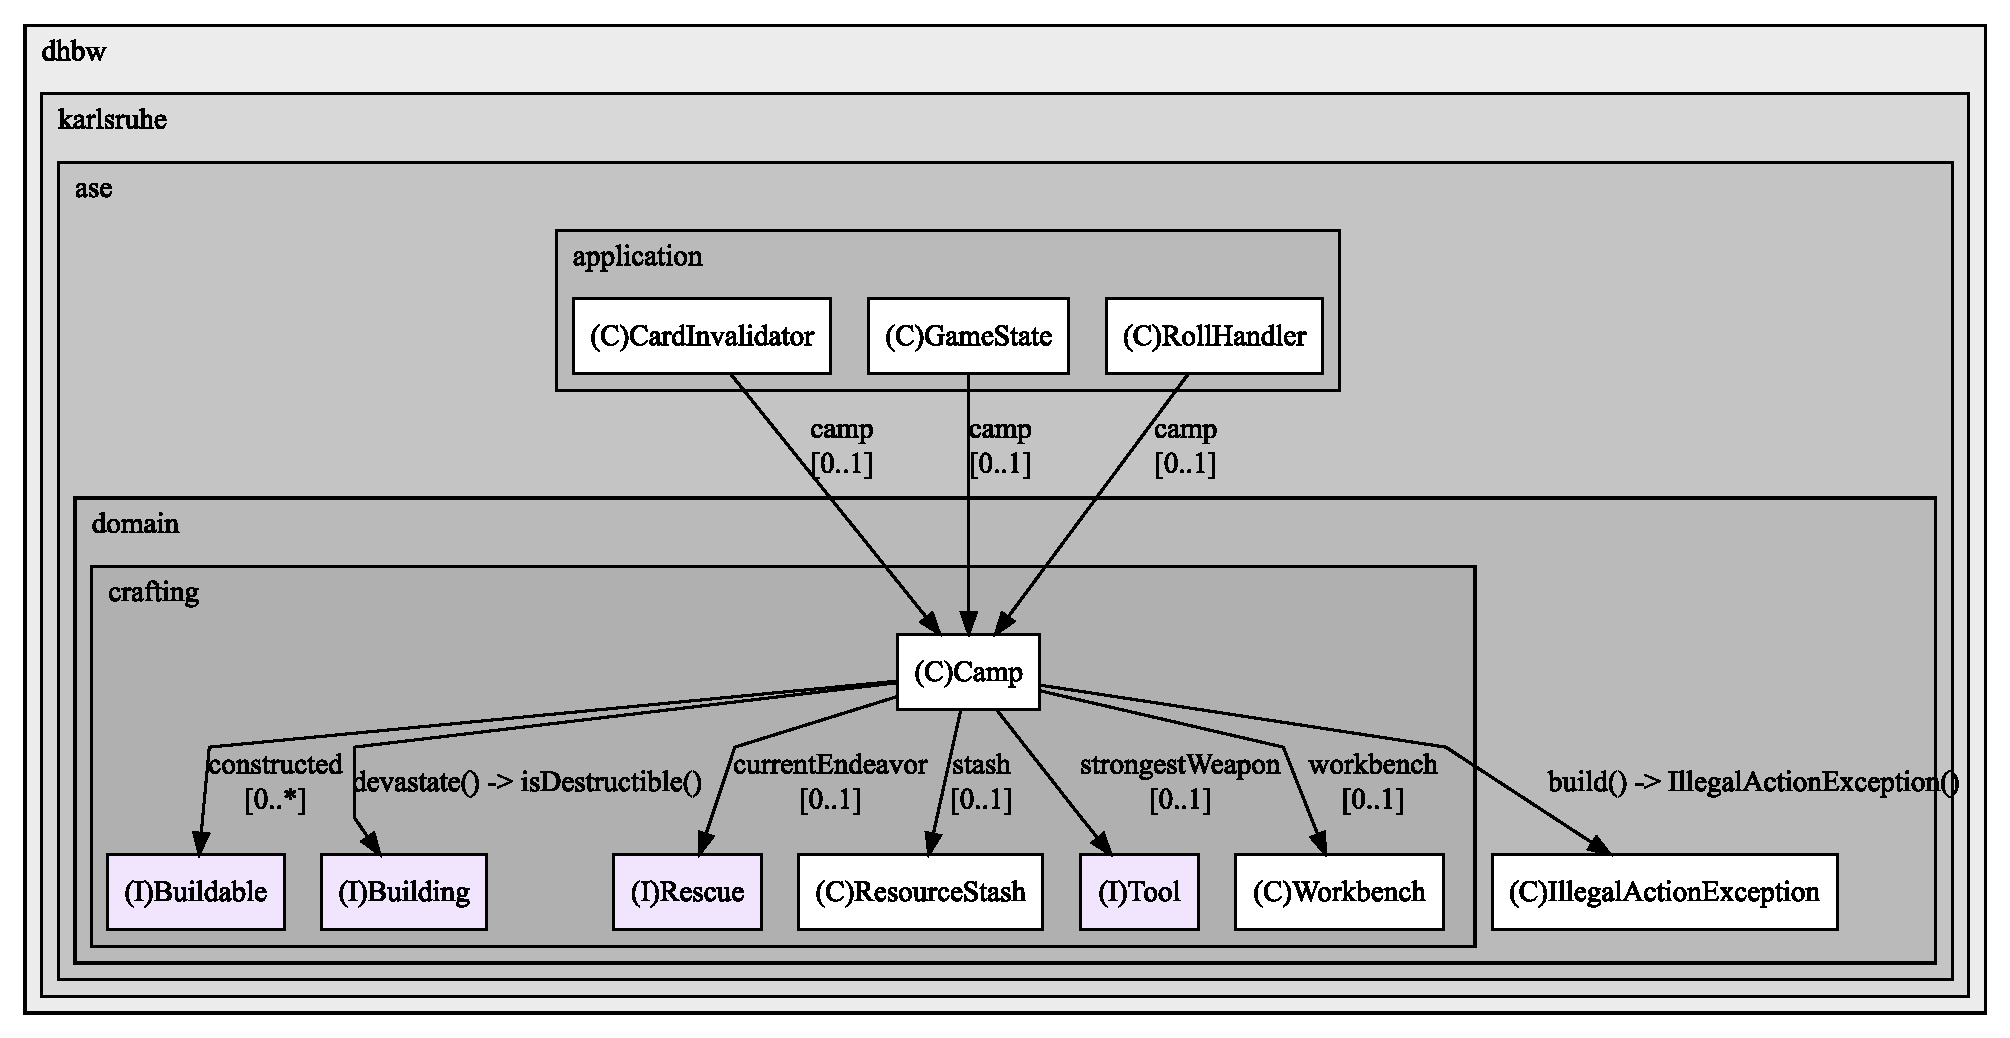
\includegraphics[width=1.\textwidth]{Bilder/Camp_structure.pdf} 
	\caption{UML-Diagramm 1 zum Einhalten der Dependency Rule von \textit{Camp}. }
	\label{fig:dep-camp}
\end{figure} 

\subsubsection{Positiv-Beispiel 2:}

\autoref{fig:dep-game} zeigt ein weiteres positives Beispiel für die Dependency Rule, 
da diese in dieser Softwarearchitektur nicht verletzt wird. Abgebildet ist die Klasse \textit{Game}, 
welche Lediglich von Klassen aus der eigenen Schicht (\textit{application}) und Klassen aus der tieferen 
Schicht \textit{domain} abhängt. Abhänig von Game sind nur Klassen aus der Schicht \textit{plugin},
bzw. dem konkreten \textit{cli}-Plugin. 

\begin{figure}[H]
	\centering
	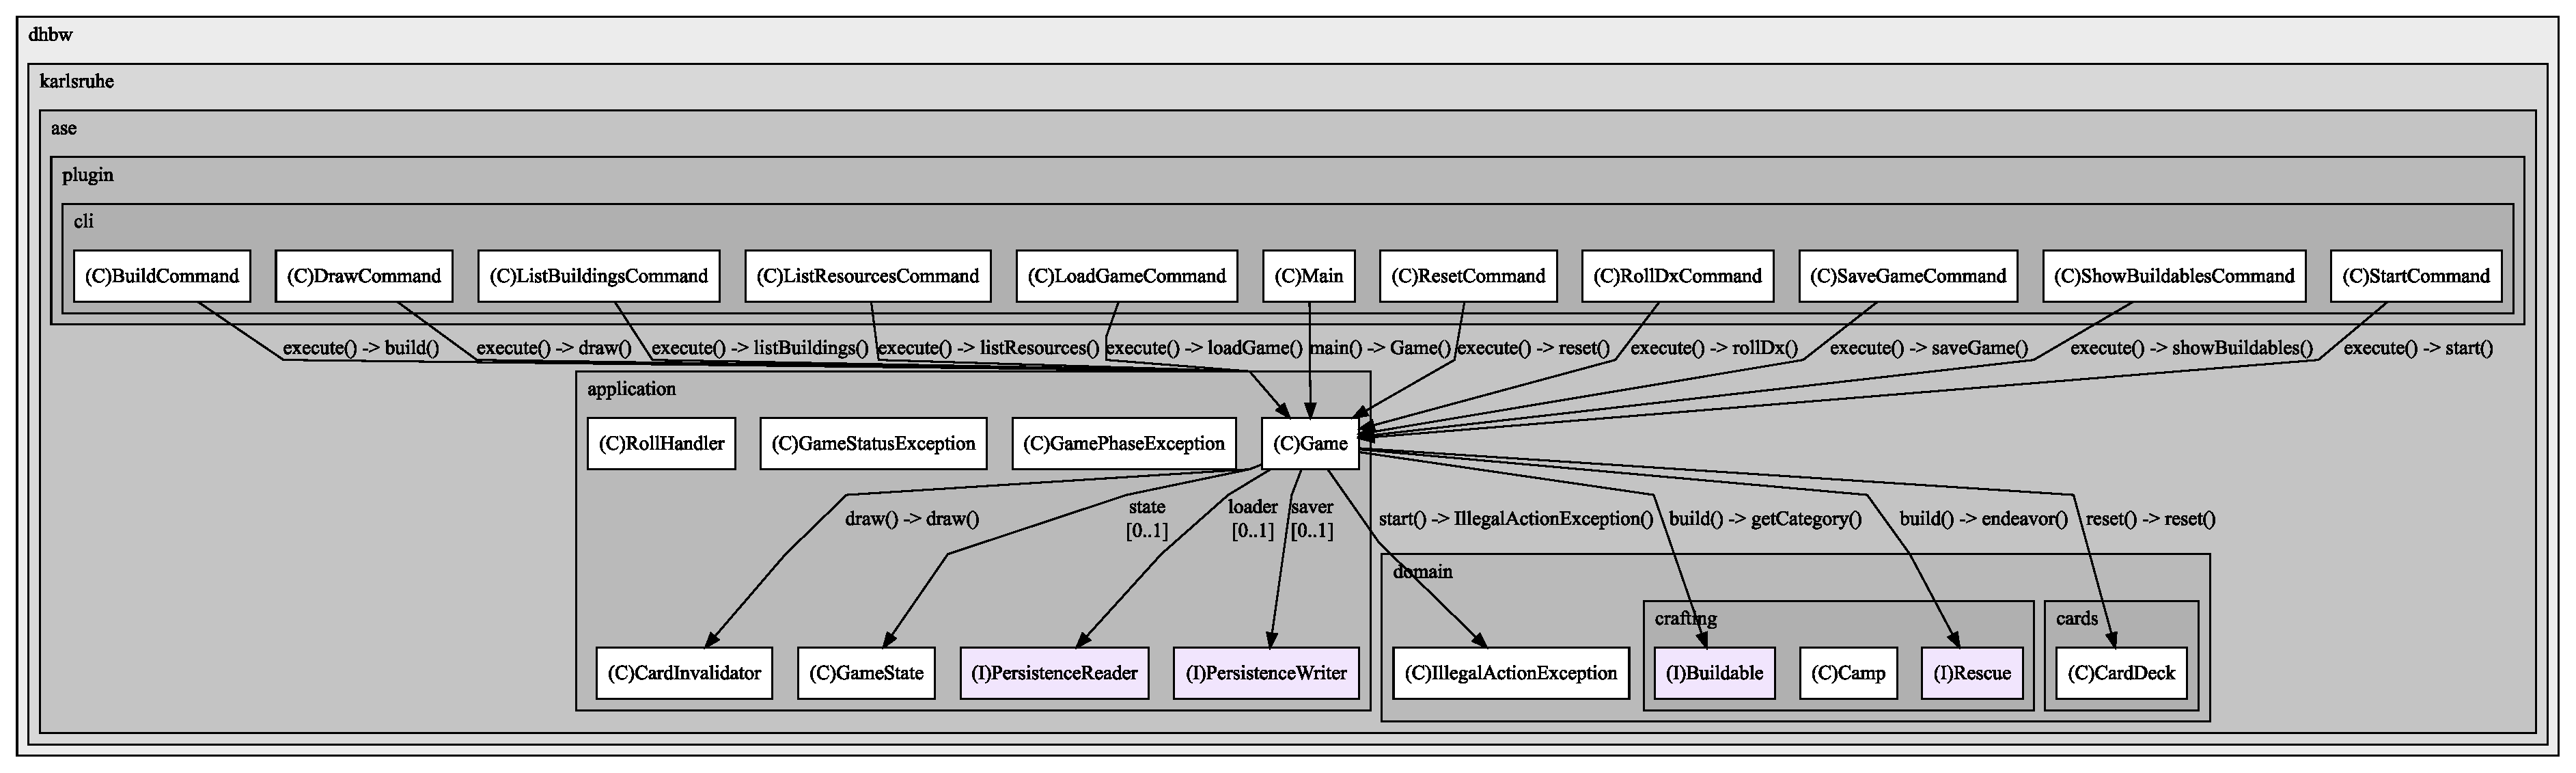
\includegraphics[width=1.05\textwidth]{Bilder/Game_structure.pdf} 
	\caption{UML-Diagramm 2 zum Einhalten der Dependency Rule von \textit{Game}. }
	\label{fig:dep-game}
\end{figure} 


\section{Analyse der Schichten} \label{sec:clean_arch:layers}

In dieser Softwarearchitektur gibt es folgende Schichten aufsteigend sortiert nach Tiefe: 
\texttt{plugin}, \texttt{application}, \texttt{domain} und \texttt{abstraction}.
Hierbei stellt \textit{plugin} die äußerste und \textit{abstraction} die tiefste Schicht dar. 

\subsubsection{Schicht Plugin:}

Bei einem Refactoring der Plugin-Schicht ist aufgefallen, dass viele der (Fehler-)Hinweise, 
die aufgrund von falschem Befehlssyntax oder einem falschen Befehl an den User über das CLI ausgegeben werden, 
keine gemeinsame einheitliche Form aufwiesen, da diese direkt als String ausgegeben wurden. 
Um eine einheitliche Fehlermeldung zu gewährleisten wurde der \textit{ErrorBuilder} eingefügt, 
dessen Aufgabe es ist, die Fehler einheitlich zu formatieren und auszugeben. \autoref{fig:layer-ErrorBuilder} 
zeigt das UML-Klassendiagramm dieser Klasse. Sie wird im gesamten CLI-Plugincode verwendet um (Fehler-)Hinweise 
auszugeben. \\
Über verschiedene Konstruktoren kann ein Grund für den (Fehler-)Hinweis und eine mögliche Abhilfeemfehlung 
eingegeben werden.
Mit der \textit{print}-Methode kann der erzeugte (Fehler-)Hinweis dann formatiert an den User ausgegeben werden. 
Hierzu wird aus Gründen der Testbarkeit an die Funktion \textit{printError} des Proxys \textit{Terminal} delegiert. \\
Diese Klasse befindet sich im Plugin-Layer (insb. im CLI-Plugin), da die konkrete Ausgabe an den User 
in Form von Text von dem CLI abhängt. Die high-level Fehlermeldungen die von den tieferen Schichten über 
Exceptions realisiert sind können von jedem Plugin anders verarbeitet und an den User weitergegeben werden. 
In der CLI funktioniert dies mit dem ErrorBuilder, während es mit einem denkbaren GUI-Plugin über bspw. 
ein Popup funktionieren könnte. Der ErrorBuilder ist lediglich für die Ausgabe an den Nutzer zuständig 
und enhält keine Fehler-Logik und gehört somit in die Plugin-Schicht. 

\begin{figure}[H]
	\centering
	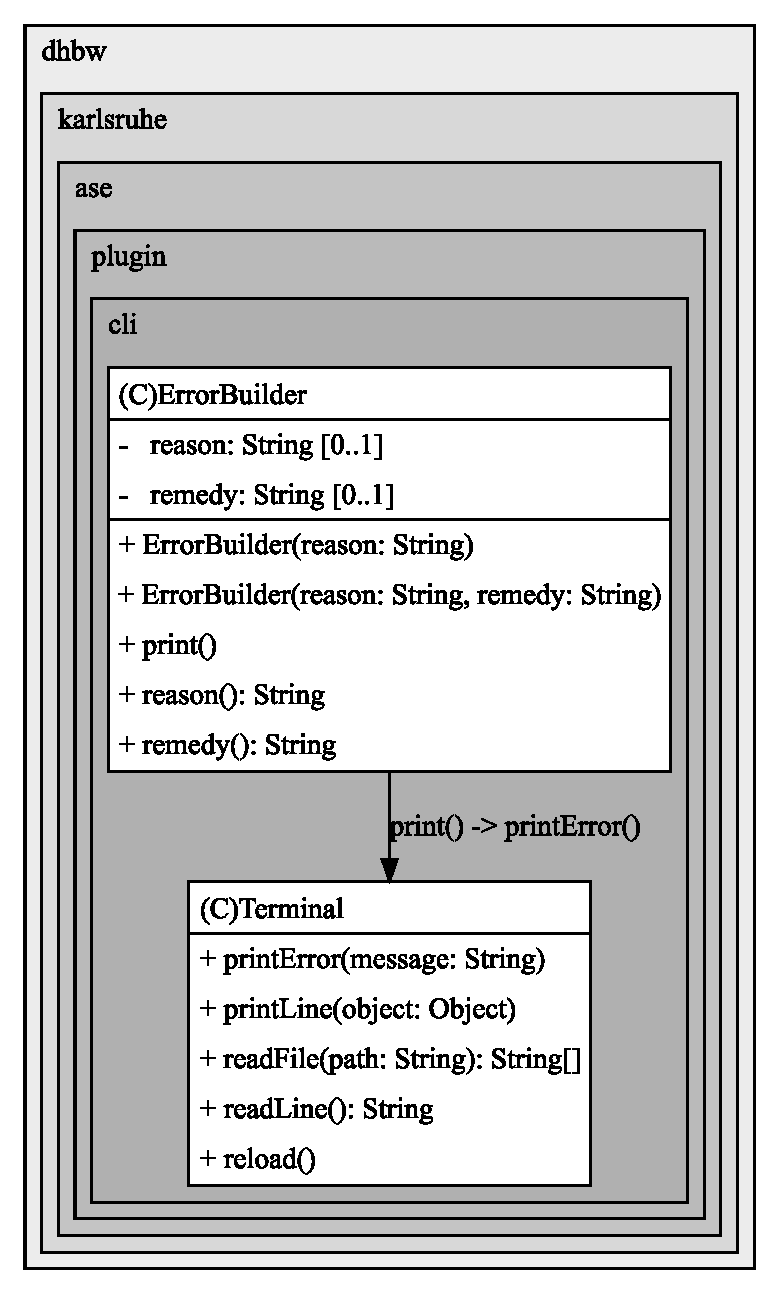
\includegraphics[width=0.5\textwidth]{Bilder/ErrorBuilder_structure.pdf} 
	\caption{Beispielklasse der Plugin-Schicht: ErrorBuilder.}
	\label{fig:layer-ErrorBuilder}
\end{figure} 

\subsubsection{Schicht Domain:}

Der \textit{ResourceStash} ist fester Teil der Domain-Schicht und stellt hier ein Wrapper mit Methodennamen 
in Domänensprache für eine Resource-Deque dar. \autoref{fig:layer-ResourceStash} zeigt das zugehörte UML-Klassendiagramm.
Der ResourceStash beinhaltet und verwaltet alle Ressourcen, die der Spieler im Verlauf des Spiels ansammelt. 
Durch eine Katastrophe oder das Verlieren gegen ein Tier wird der ResourceStash zerstört (\textit{devastate})
und alle ungeschützten Ressourcen gelöscht. Das Erbauen eines \textit{Shack}s\footnote{nicht in der Abb.} 
erlaubt es die obersten $n \in [0;\inf)$ Ressourcen zu schützen (\textit{protectTopMostNResources}), 
sodass diese nach einem \textit{devastate} übrig bleiben. Zusätzlich können Ressourcen hinzugefügt,
konsumiert oder deren Vorhandensein überprüft werden. \textit{Camp} und \textit{Workbench} teilen 
sich eine Referenz auf denselben Stash. \\
Die Klasse ist als Teil des Kartenspiels (der Domäne) im Code natürlich in der Domain-Schicht angesiedelt und 
wird von anderen Domänenklassen genutzt. Es gibt keine Möglichkeit die Klasse in einer der anderen Schichten 
sinnvoll anzusiedeln.

\begin{figure}[H]
	\centering
	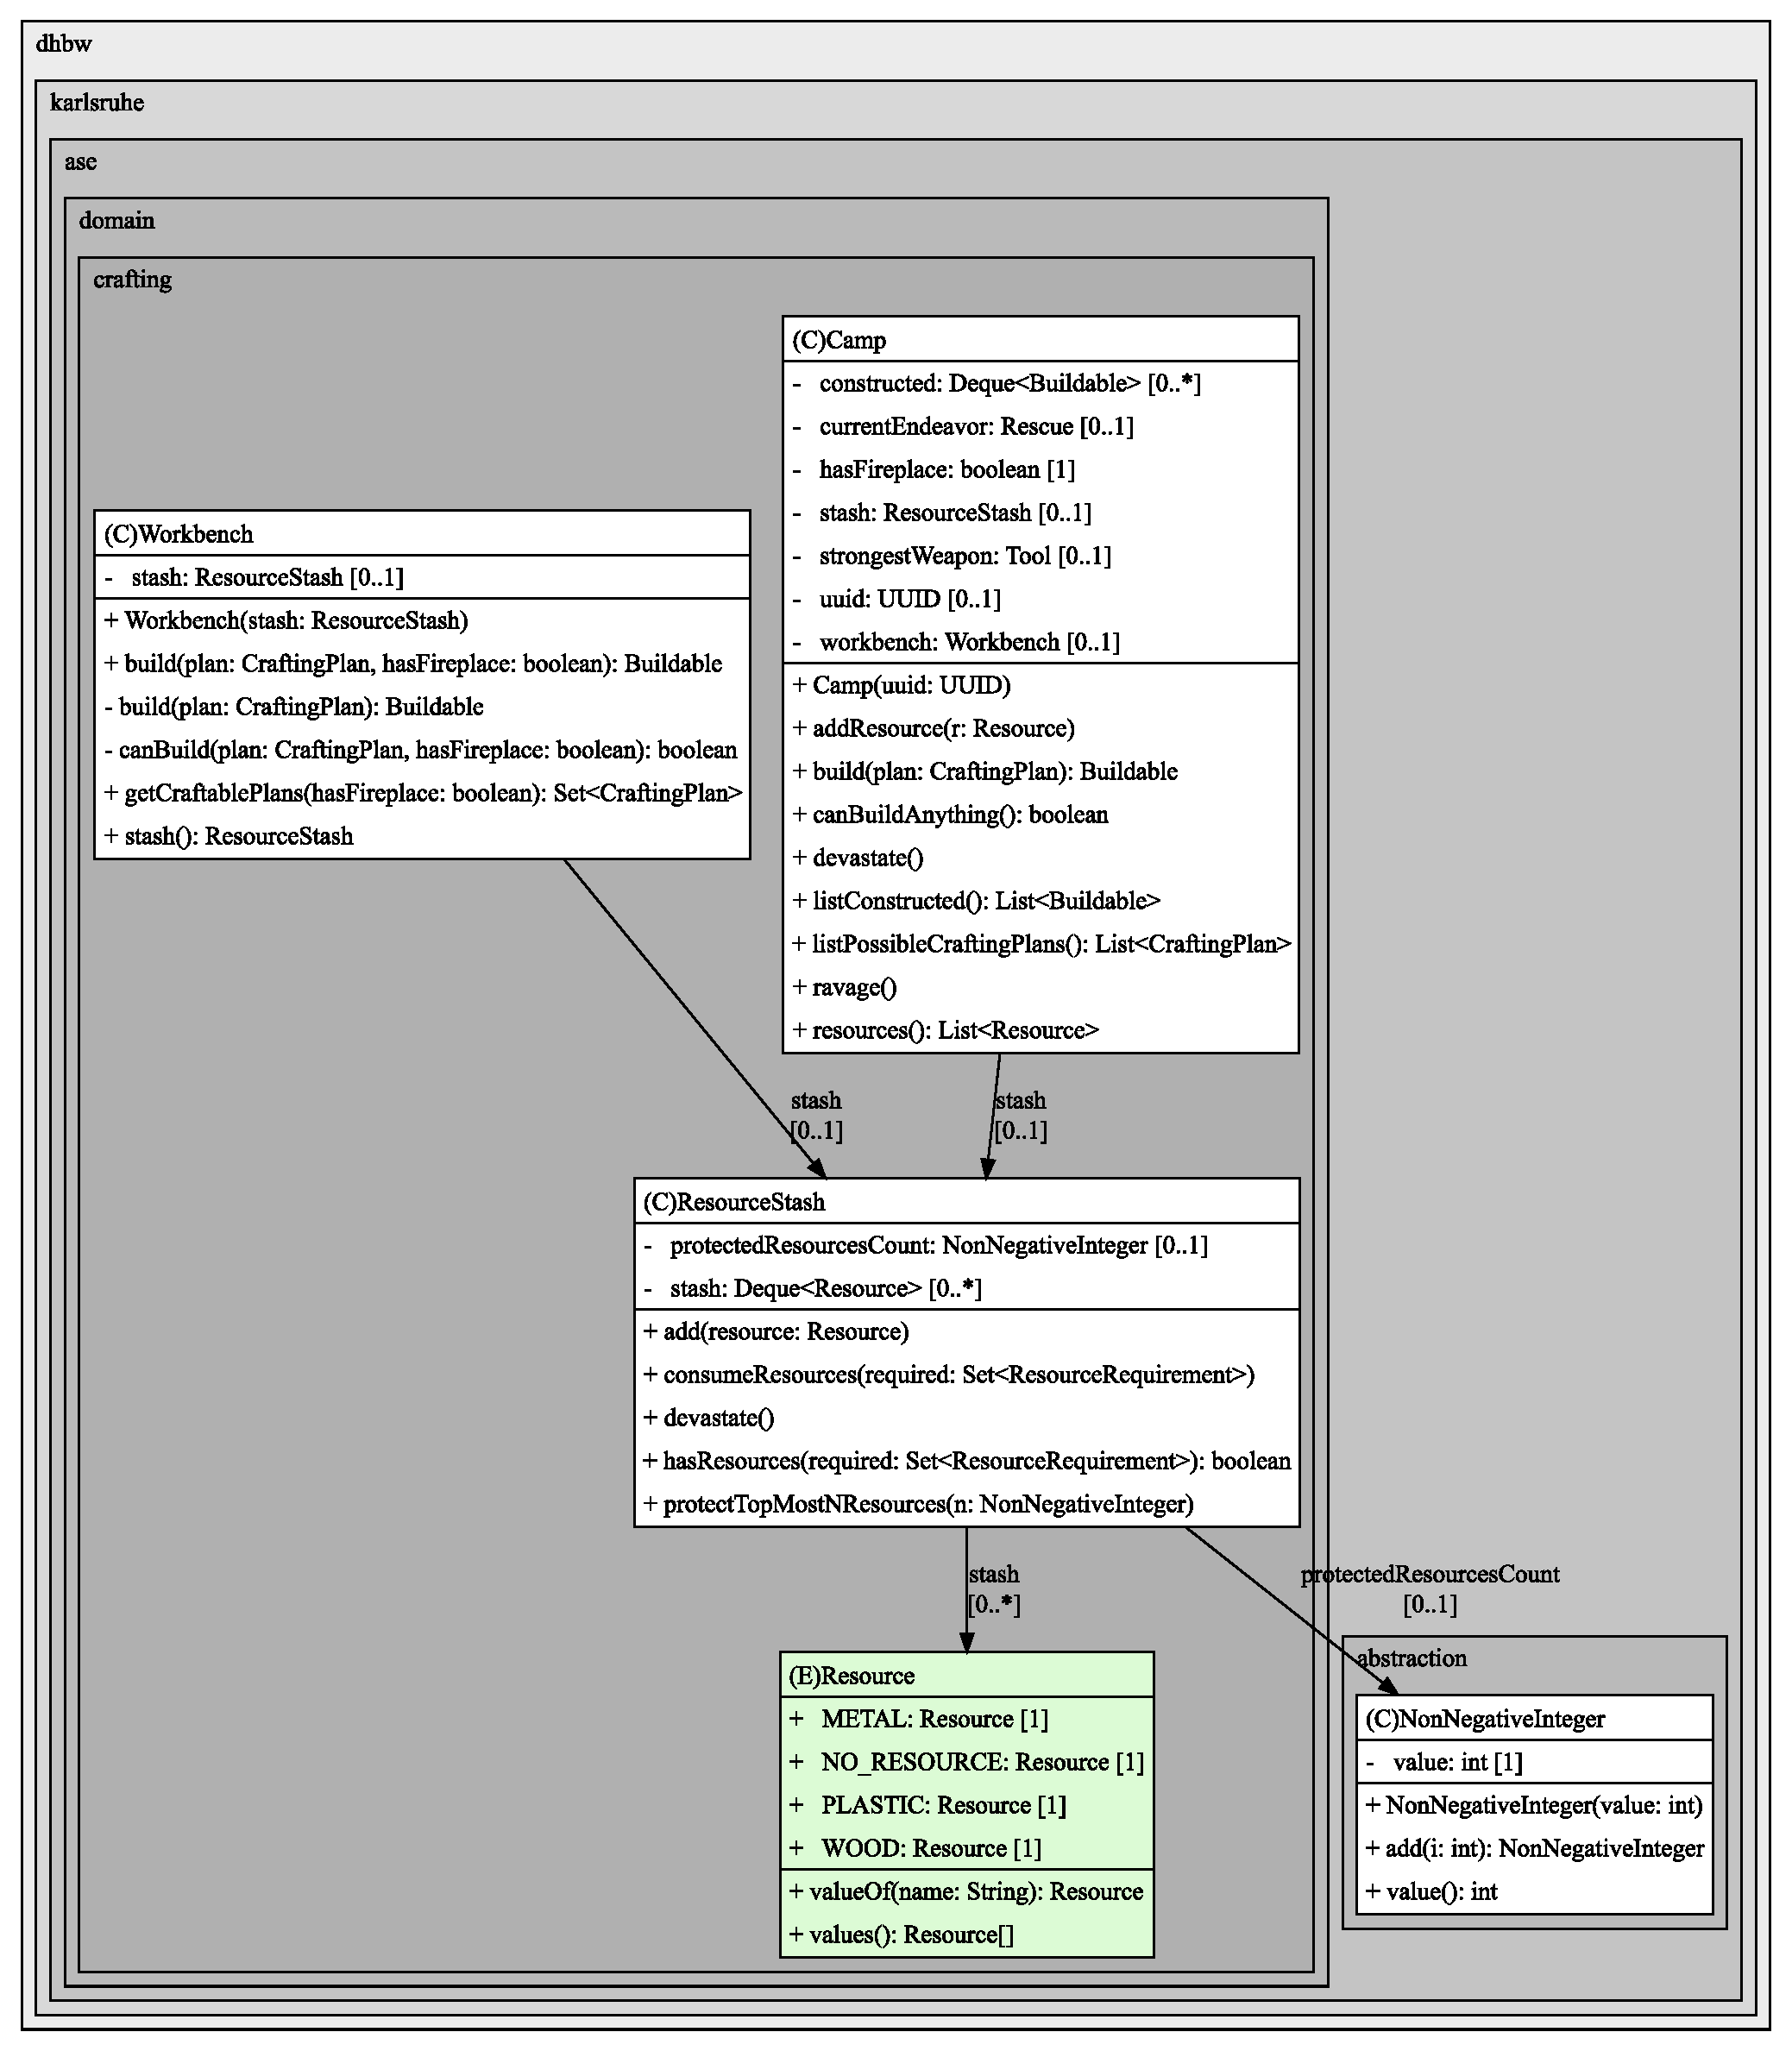
\includegraphics[width=1.05\textwidth]{Bilder/ResourceStash_structure.pdf} 
	\caption{Beispielklasse der Domain-Schicht: ResourceStash.}
	\label{fig:layer-ResourceStash}
\end{figure} 